\section{Fogen, Felder und Listen}
\rule{\textwidth}{0.4pt}
\paragraph{Folgen}
spielen in der Informatik eine Überragende Rolle. Das sieht man schon an der Vielzahl von Begriffen: Folge, \textbf{Feld}, Schlange, \textbf{Liste}, Datei, Stapel, Zeichenkette, Log, \(\cdots\). Wir unterscheiden:
\begin{itemize}
    \item \textbf{abstrakter} Begriff [2, 3, 5, 7, 9, 11, \(\cdots\)] - Mathe
    \item Funktionalität (stack, \(\cdots\)) - Softwaretechnik
    \item Repräsentation - Algorithmik
\end{itemize}

\paragraph{Anwendungen}
\(\cdots\)
\paragraph{Form Follows Function} 

\begin{center}
    
\begin{tabular}{l|c c c c|l}
    Operation & LIST & SLIST & UArray & CArray & explanation\\
    \hline
    $[\cdot]$ & n & n & 1 & 1 & \\
    $|\cdot|$ & $1^*$ & $1^*$ & 1 & 1 & not with inter-list \\
    FIRST & 1 & 1 & 1 & 1 \\
    LAST & 1 & 1 & 1 & 1 \\
    INSERT & 1 & $1^*$ & n & n & InsertAfter only\\
    REMOVE & 1 & $1^*$ & n & n & RemoveAfter only\\
    PUSHBACK & 1 & 1 & $1^*$ & $1^*$ & amortized \\
    PUSHFRONT & 1 & 1 & n & $1^*$ & amortized \\
    POPBACK & 1 & n & $1^*$ & $1^*$ & amortized \\
    POPFRONT & 1 & 1 & n & $1^*$ & amortized \\
    CONCAT & 1 & 1 & n & n \\
    SPLICE & 1 & 1 & n & n \\
    FINDNEXT & n & n & $n^*$ & $n^*$ & cache-efficient \\
\end{tabular}
\end{center}

\newpage

\subsection{Verkettete Listen}
Eine verkettete Liste ist eine häufig verwendete Art von Datenstruktur, bei der jedes Element in der Liste Informationen über das nächste Element enthält. Es gibt verschiedene Arten von verketteten Listen, darunter einfach verkettete Listen und doppelt verkettete Listen.

\subsubsection{Doppelt verkettete Listen}
Bei doppelt verketteten Listen enthält jedes Listenelement Informationen sowohl über das vorherige als auch das nächste Element. Dies ermöglicht eine effiziente Navigation in beide Richtungen innerhalb der Liste.

In der Vorlesung haben wir eine Implementierung von doppelt verketteten Listen betrachtet. Jedes Listenelement wird durch die Klasse "Item" repräsentiert. Ein Item enthält zwei Handles (Zeiger) auf die vorherigen und nächsten Elemente in der Liste sowie ein Element selbst, das den eigentlichen Datenwert enthält.

Hier ist die Definition der Klasse "Item":


\paragraph{Listenglieder (Items)}
\begin{verbatim}
    Class Handle = Pointer to Item
    Class Item of Element // one link in a doubly linked list
        e : Element
        next : Handle 
        prev : Handle
        invariant next→prev = prev→next = this
\end{verbatim}

\begin{center}
    \centering
    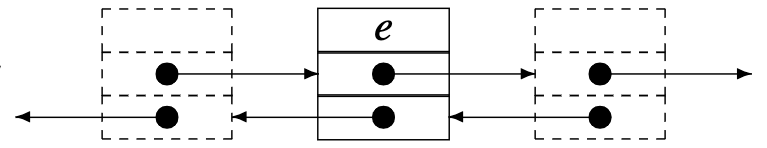
\includegraphics[width=0.5\textwidth]{folgen-felder-listen/abb_1.png}
    \label{fig:abb_1}
\end{center}

\subparagraph{Probleme:}

\begin{itemize}
    \item \textbf{Vogränger des ersten} Listenelements?
    \item \textbf{Nachfolger des letzten} Listenelements?
\end{itemize}

\newpage
    
\begin{center}
    \centering
    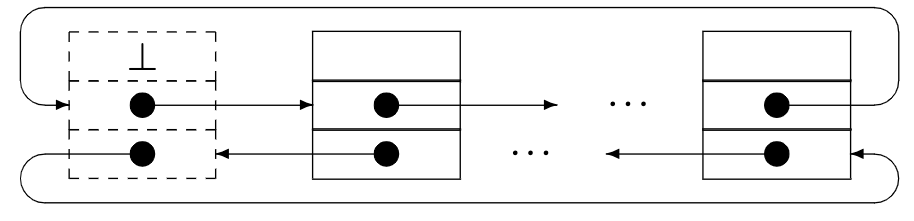
\includegraphics[width=0.5\textwidth]{folgen-felder-listen/abb_2.png}
    \label{fig:abb_2}
\end{center}

\paragraph{Trick: Dummy-Header}
Der Trick mit dem Dummy-Header ist ein nützliches Werkzeug zur Verbesserung der Implementierung und Verwendung von Listenstrukturen. Er steigert Lesbarkeit, Effizienz und Eleganz des Codes und erleichtert das Testen. Durch Vermeidung von Sonderfällen und Aufrechterhaltung der Invariante der verketteten Liste gewährleistet der Dummy-Header reibungslose und zuverlässige Listenoperationen.\\
Der Dummy-Header ist eine Technik zur Vereinfachung der Implementierung von Listenstrukturen. Durch Verwendung eines speziellen Listenelements am Anfang und Ende der Liste können viele Sonderfälle vermieden werden. Er dient als Platzhalter und Verweis für den Anfang und das Ende der Liste.\\
Der Dummy-Header bietet folgende Vorteile bei der Verwendung von Listen:

\begin{itemize}
    \item [+]Die Invariante der verketteten Liste wird immer erfüllt. Der Dummy-Header stellt sicher, dass es immer einen Vorgänger für das erste Element und einen Nachfolger für das letzte Element gibt.
    
    \item [+]Durch Vermeidung vieler Sonderfälle wird die Implementierung einfacher, lesbarer und eleganter. Es müssen keine zusätzlichen Bedingungen für leere Listen oder Listen mit einem einzigen Element überprüft werden.
    
    \item [+]Der Zugriff auf das erste und letzte Element der Liste ist effizient und erfordert keine aufwändige Traversierung der gesamten Liste.
    
    \item [+]Der Dummy-Header erleichtert das Testen der Listenimplementierung, da die speziellen Fälle von leeren Listen und Listen mit einem einzigen Element bereits abgedeckt sind.
    \item [-]Der zusätzliche Speicherplatz, der für den Dummy-Header benötigt wird. Dieser Faktor ist in der Regel vernachlässigbar, besonders bei längeren Listen.

\end{itemize}


Die Definition der Listenklasse mit dem Dummy-Header lautet:

\begin{verbatim}
    class List of Element {
        // Item h ist der Vorgänger des ersten Elements und der Nachfolger des letzten Elements
        // Pos. vor jedem eigentlichen Element

        // !help
    
        // Einfache Zugriffsfunktionen
        Function head: Handle; return Adresse von h
        Function isEmpty: {0, 1}; return h.next = head // 〈〉?
        Function first: Handle; assert ¬isEmpty; return h.next
        Function last: Handle; assert ¬isEmpty; return h.prev
    }
\end{verbatim}
\begin{verbatim}
    Procedure splice(a,b,t : Handle) {
        //!help
    }
\end{verbatim}

\paragraph{Der rest sind Einzeiler (?)}

\begin{verbatim}
    // Moving elements around within a sequence.
    // 〈... , a, b, c ... , a', c', ...〉 → 〈... , a, c ... , a', b, c', ...〉
    Procedure moveAfter(b, a' : HANDLE) splice(b, b, a')
    Procedure moveToFront(b : HANDLE) moveAfter(b, HEAD)
    Procedure moveToBack(b : HANDLE) moveAfter(b, LAST)
\end{verbatim}

\paragraph{Oder doch nicht? Speicherverwaltung!}
Die Speicherverwaltung in einer Programmiersprache kann potenziell sehr langsam sein. Ein Beispiel dafür ist eine Variable, die einmal erstellt wurde, wie zum Beispiel ein statisches Element in Java.
Die \textit{FREELIST} enthält ungenutzte Elemente, während \textit{CHECKFREELIST} sicherstellt, dass sie nicht leer ist.
In realen Implementierungen gibt es verschiedene Ansätze:
\begin{enumerate}
\item Ein naiver Ansatz, der jedoch eine gute Speicherverwaltung bietet.
\item Verfeinerte Konzepte zur Verwaltung der \textit{FREELIST}, die über Klassen hinweg angewendet werden können und die Freigabe von Elementen ermöglichen.
\item Anwendungsspezifische Ansätze, zum Beispiel wenn man im Voraus weiß, wie viele Elemente insgesamt benötigt werden.
\end{enumerate}

\paragraph{Items Löschen}
\begin{verbatim}
    // 〈... , a, b, c, ...〉 7 → 〈... , a, c, ...〉
    Procedure remove(b : HANDLE) moveAfter( b, freeList.head)
    Procedure popFront remove(FIRST)
    Procedure popBack remove(LAST)
\end{verbatim}
\paragraph{Elemente einfügen}
\paragraph{Ganze (Teil)Listen Manipulieren}
\paragraph{Suchen}
\paragraph{Funktionalität \(\leftrightarrow\) Effizienz}
Wir betrachten folgendes Beispiel um Listenlängen zu verwalten. Neben den vorhandenen Elementen verfügt die Liste nun auch über eine zusätzliche Eigenschaft namens \texttt{SIZE}.\\
\textbf{Problem:} inter-list SPLICE geht nicht mehr in konstanter Zeit.
Die Moral dabei ist das es keine perfekte Art, Listen zu implementieren gibt. Es hängt von den spezifischen Anforderungen und den gewünschten Operationen ab.

\newpage

\subsubsection{Einfach verkettete Listen}
\begin{center}
    \centering
    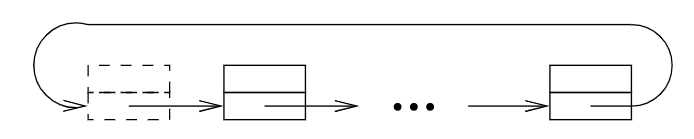
\includegraphics[width=0.5\textwidth]{folgen-felder-listen/abb_3.png}
    \label{fig:abb_2}
\end{center}

Vergleich mit doppelt verketteten Listen
\begin{itemize}
    \item weniger Speicherplatz
    \item Platz ist oft auch Zeit
    \item eingeschränkter, z. B. kein remove
    \item merkwürdige Benutzerschnittstelle, z. B. removeAfter
\end{itemize}
\paragraph{Einfach verkettete Listen – Invariante?}
\paragraph{Einfach verkettete Listen – SPLICE}
\paragraph{Einfach verkettete Listen – PUSHBACK}
\paragraph{Listen: Zusammenfassung, Verallgemeinerungen}
\paragraph{Felder (Arrays)}
\subparagraph{Beschränkte Felder (Bounded Arrays)}
\subsection{Unbeschränkte Felder (Unbounded Arrays)}
\paragraph{Unbeschränke Felder – Anwendungen}
\paragraph{Unbeschränke Felder – Grundidee}
\paragraph{Unbeschränke Felder
mit teilweise ungenutztem Speicher}
\paragraph{Kürzen}
\subsubsection{Amortisierte Komplexität unbeschr. Felder}
\paragraph{Beweis: Konto-Methode (oder Versicherung)}
\subsection{Amortisierte Analyse – allgemeiner}
\paragraph{Amortisierte Analyse – Diskussion}
\subsection{Stapel und Schlangen}
\subsection{Vergleich: Listen – Felder}
\paragraph{Iterieren}
\paragraph{Einfügen an zufälliger Position}
\paragraph*{Ausblick: Weitere Repräsentationen von Folgen}


